\chapter{Continous Integration}


Have you ever had a situation when your software has a bug but it is
not discovered for a long time?  The existence of the bug and its
ability to escape detection may surprise your entire team. ``How did
that happen?'', you may ask.  This may happen due to a wide variety of
reasons. One of the possible reasons is that the software has not been
well tested and as a result the bug is not detected. Testing is an
important method detecting bugs.  However, testing can be tideous.  It
is common that someone makes a ``small'' change and skips testing.
The person believes the change is so small and cannot possibly have
any bug.  If several people add a few small changes here and there,
the software soon is full of ``small'' bugs.  Why do people not test
their programs immediately after they have made changes?  One reason
is that testing require additional work.

Is it possible testing is fully automated without any additional
effort? {\it Continuous Integration} (CI) does exactly that.

You still need to write testers. There is no way avoiding that part.
What continuous integration does is to automatically invole these
testers whenver you push your program to the shared repository.
This chapter uses {\tt Travis-CI} for continuous integration. Before explaining how
to use Continuous Integration, it is necessary first explaining how Python
testing works.

\section{Limitations of Testing}

It is important understanding that testing has limitations.  It is
practically impossible testing every possible scenario.  Every {\tt
  if} is a {\it condition}. A condition divides a program into two
different paths depending whether the condition is true or not.  A
non-trivial program can easily have hundreds of conditions.  As a
simple explanation why it is not possible testing every possible
scenario. Let's consider a program with 100 {\it independent}
conditions, i.e., whether condition is true or false does not affect
any other condition.  There are $2^{100}$ possible scenarios.  The
fastest computer in the world can perform several hundred quadrillion
($10^{15}$) calculations per second; this is a parallel computer but
let's not worry about that detail.  Because $\log_2(10) \approx 3.3$,
$10^{15} \approx 2 ^ {50}$. Thus, the fastest computer can check as
many as $2 ^ {50}$ conditions per second. How many can this computer
check per minute? $2 ^ {50} \times 60$. How about a day (86,400
seconds)?  $2 ^ {50} \times 86400 \approx 2 ^ {66}$.  In order to test
$2^{100}$ possible scenarios, this computer needs to work $2^{34}$
days; this is very long time (much longer than the history of humans).
In fact, the situation is even worse.  The estimation above considers
only two possible cases for each condition: true or false. If the
condition compares two numbers, then ``every possible scenario'' means
every possible pairs of these two numbers.  What does this mean? It
would be completely impossible testing every possible scenario of a
program's execution paths controlled by the conditions.

Does this mean there is no need to test because it is not possible
testing all possible scenarios? No. What it means is that testing has to
be done carefully so that testing can detect as many problems (i.e.,
bugs) as possible.  Good tests should consider many different scenarios.

\section{Structure of Tests}

\marginnote{Do not put {\tt assert} in your production code.}

Many books talk about the importance of testing and how to write
tests.  However, few books talk about how to structure tests. Before
writing any test, you need to answer a fundamental question: do you
want the testing code to be sent to the users (or customers)?  In most
cases, the answer is no.


\section{Pytest}





\begin{figure}[h] \centering
{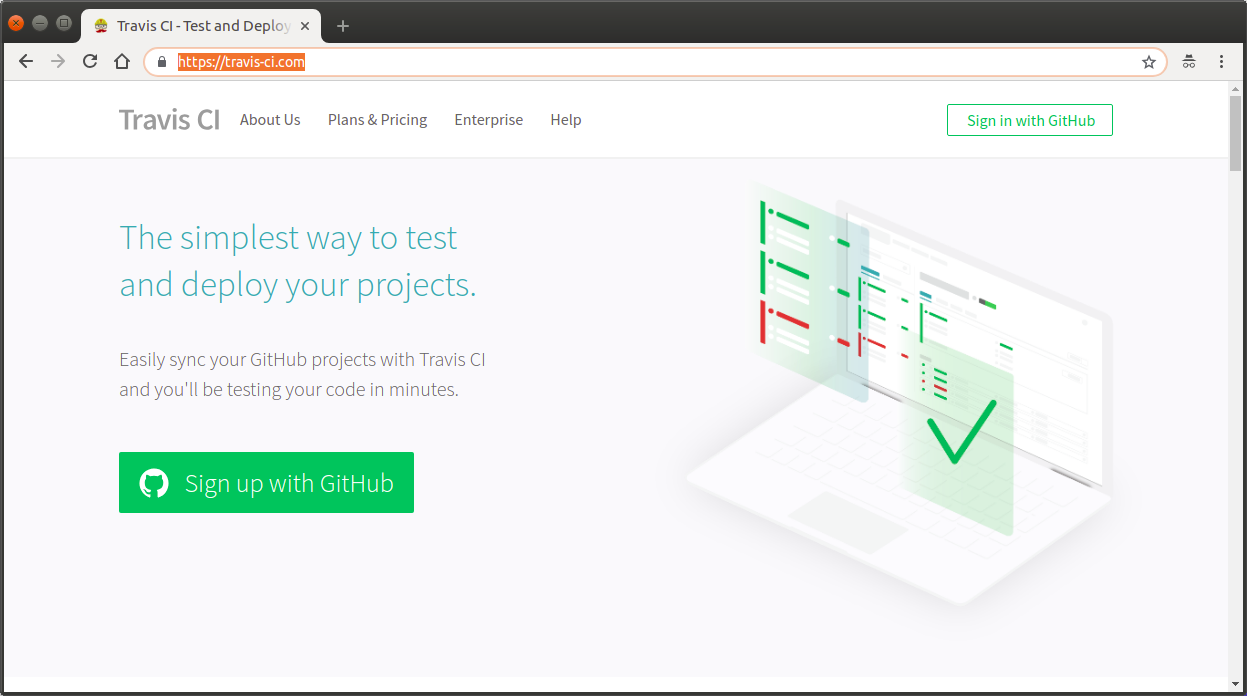
\includegraphics[width=4.5in]{\thischapterpath/figures/travis01.png}}
\caption{Travis-CI.com is a website supporting continuous integration.}
\label{fig:travis01}
\end{figure}
